\begin{figure}[H]
    \begin{subfigure}{.49\textwidth}
        \centering
        \caption*{$u(x_1, x_2) = x_1^{\frac{1}{3}} x_2^{\frac{2}{3}}$}
        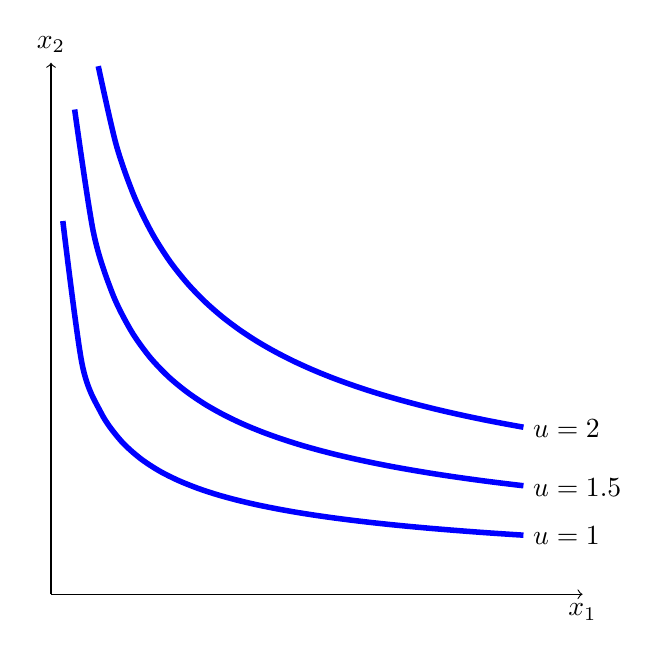
\begin{tikzpicture}[scale=1.5]
            \draw[->] (0, 0) -- (4.5, 0) node[below] {$x_1$};
            \draw[->] (0, 0) -- (0, 4.5) node[above] {$x_2$};
            \draw[domain=0.1:4, smooth, variable=\x, blue, line width=2pt] plot ({\x}, {1/(\x^0.5)});
            \draw[domain=0.2:4, smooth, variable=\x, blue, line width=2pt] plot ({\x}, {1.5^1.5/(\x^0.5)});
            \draw[domain=0.4:4, smooth, variable=\x, blue, line width=2pt] plot ({\x}, {2^1.5/(\x^0.5)});
            \node[right] at (4,0.5) {$u = 1$};
            \node[right] at (4,0.9) {$u = 1.5$};
            \node[right] at (4,1.4) {$u = 2$};
        \end{tikzpicture}
    \end{subfigure}
    \begin{subfigure}{.49\textwidth}
        \centering
        \caption*{$u(x_1, x_2) = x_1 x_2$}
        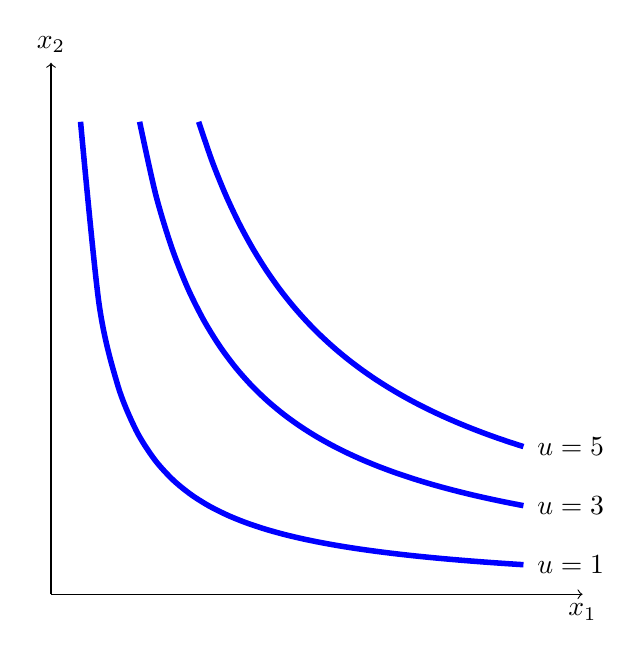
\begin{tikzpicture}[scale=1.5]
            \draw[->] (0, 0) -- (4.5, 0) node[below] {$x_1$};
            \draw[->] (0, 0) -- (0, 4.5) node[above] {$x_2$};
            \draw[domain=0.25:4, smooth, variable=\x, blue, line width=2pt] plot ({\x}, {1/\x});
            \draw[domain=0.75:4, smooth, variable=\x, blue, line width=2pt] plot ({\x}, {3/\x});
            \draw[domain=1.25:4, smooth, variable=\x, blue, line width=2pt] plot ({\x}, {5/\x});
            \node at (4.4,0.25) {$u = 1$};
            \node at (4.4,0.75) {$u = 3$};
            \node at (4.4,1.25) {$u = 5$};
        \end{tikzpicture}
    \end{subfigure}
\end{figure}
